%
% !TEX root = Main.tex 


\section{Experiments in the stochastic setting} 
\label{app:Exp}
%
After the theoretical main course, we propose an experimental dessert.
%We propose a few simple experiments to illustrate our theoretical analysis. 
We  reuse the experimental setups of~\cite{Audibert10BA} in Experiments~\ref{fp:A} to~\ref{fp:G}. We only consider Bernoulli distributions and the optimal arm  has always mean
$1/2$. Each experiment corresponds to a different situation for the gaps. They are either clustered in a few groups
or distributed according to an arithmetic or geometric progression. Experiment~\ref{fp:H} reuses the `square-root gap' scenario when $\complexityBoth = \sqrt{2K}\complexitySR$ as detailed in Remark~\ref{rem:LOWbobCOMP}. The experimental setups are given below. %\todom{no reference from the main paper}
%\todom{adversarial experiments}
%\todom{did Peter Auer give any experiments}
\begin{itemize}[leftmargin=*]
	\item[] 
	\begin{fp}{fp:A}{}
\textit{One group of bad arms},
	$K= 20$, $\mu_{2:20}= 0.4 \equiv \forall j\in \{2,\ldots,20\}, \mu_j= 0.4$
\end{fp}
	%Experiment 1: 
		\item[]  \begin{fp}{fp:B}{} \textit{Two groups of bad arms},
	$K	= 20$, $\mu_{2:6} =  0.42$, $\mu_{7:20} =  0.38$.\end{fp}
		\item[] \begin{fp}{fp:C}{} \textit{Geometric progression},
	$K	= 4$, $\mu_{i} = 0.5 -(0.37)^i$, $i\in \{2,	3,4\}$ \end{fp}
		\item[] 	\begin{fp}{fp:D}{}
	\textit{6
	arms divided into three groups},	
	$K	= 6$, $\mu_2 = 0.42$, 	$\mu_{3:4}= 0.4$, $\mu_{5:6}= 0.35$\end{fp}
		\item[] 	\begin{fp}{fp:E}{} \textit{Arithmetic progression},
	$K 	= 15$, $\mu_i= 0.5 -0.025i$, $i\in \{	2,\ldots,15\}$ \end{fp}
		\item[] 	\begin{fp}{fp:F}{} \textit{2 good arms and a large group of bad arms}, $K= 20$, $\mu_2 = 0.48$, $\mu_{3:20}= 0.37$\end{fp}
		\item[]  	\begin{fp}{fp:G}{} \textit{Three groups of bad arms},
	$K = 30$, $\mu_{2:6}	= 0.45$, $\mu_{7:20} = 0.43$,
	$\mu_{21:30}= 0.38$	 \end{fp}
			\item[]  \begin{fp}{fp:H}{} \textit{Square-root gaps}
			$K	= 100$, $\mu_{i} = 0.5 - 0.25\sqrt{i/(2K)}$, $i\in [1:100]$ \end{fp}
\end{itemize}
In Table~\ref{tabloo}, we report the complexities $\complexitySR$, $\complexityBoth$, and $\complexityUnif$ computed in these experimental setups. Unsurprisingly, in Experiments~\ref{fp:A}, \ref{fp:C}, and~\ref{fp:E} we recover $\complexitySR=\complexityBoth$ and in Experiment~\ref{fp:H}, we have $\complexityBoth = \sqrt{2K}\complexitySR$. Experiments~\ref{fp:B}, \ref{fp:D}, \ref{fp:F}, and~\ref{fp:G} then give an idea about the behavior of  $\complexitySR$, $\complexityBoth$, and  $\complexityUnif$ with respect to each other. %  \todom{why we call it Canonical problems and the paper?} 
%\todom{lets have the background colors of the 3 columns  same as in graphs}
\begin{table}[H]
		\center
\begin{tabular}{|>{\columncolor[gray]{.97}}l>{\columncolor{pearDark!30}}r
		>{\columncolor{pearThree!30}}r
		>{\columncolor{pearTwo!30}}r|}
	\hline 
	\cellcolor{gray!40}\textbf{Experimental setup} & \cellcolor{pearDark!70}$\boldsymbol{\textcolor{white}{\complexitySR}}$ & \cellcolor{pearThree!70}$\boldsymbol{\textcolor{white}{\complexityBoth}}$ & \cellcolor{pearTwo!70}$\boldsymbol{\textcolor{white}{\complexityUnif}}$\\
	\hline
	\ref{fp:A}. One group of bad arms& 2000 & 2000 & 2000 \\
	\ref{fp:B}. Two groups of bad arms &1389 & 2083 & 3125\\
	\ref{fp:C}.	Geometric progression& 5540 & 5540 & 11080\\
	\ref{fp:D}. 6 	arms divided into three groups &400 & 500 & 938\\
	\ref{fp:E}.	Arithmetic progression& 3200 & 3200 & 24000\\
	\ref{fp:F}. 2 good arms and a large group of bad arms &5000 & 7692 &50000\\
	\ref{fp:G}.	Three groups of bad arms &4082 & 5714 & 12000\\
	\ref{fp:H}.	Square-root gaps &3200 & 22627 & 160000\\
	\hline
\end{tabular}
\caption{Comparing complexities  $\complexitySR$, $\complexityBoth$, and  $\complexityUnif$.}
\label{tabloo}\vspace{-.4cm}
\end{table}
\noindent
In Figure~\ref{exp}, we report the average success rate (which is an estimate of the probabilities of error) of~\SR, \Pone, and the \textit{static uniform allocation} on the 8 experimental problems previously detailed. The static uniform allocation is not the algorithm \RULE. \RULE{} samples an arm uniformly at random while the \textit{static} uniform allocation
simply allocates $n/K$ pulls to each arm deterministically.
The empirical results follow very closely our theoretical findings as the empirical behavior in Figure~\ref{exp} mimics the behavior of the complexities in Table~\ref{tabloo}. As~\cite{Audibert10BA}, we chose horizon~$\timeHorizon$ to be of the order of the complexity $\complexity_1=\sum_{k\in\setArms}(1/\gap^2_k),$ where $\complexitySR\leq\complexity_1\leq\complexitySR\log\nArms.$

%Note that, inspired by \Pone, one can design a sibling \textit{static} algorithm where the arm pulled at round $t$ would be $\pulledArm_t=\arg\min\limits_{k\in\setArms}  \tilde{\langle k \rangle}^{\vphantom{X}}_t \pullsNumber_{k}(t)$.
%This is a simple anytime and parameter free algorithm designed specially for the stochastic case. This algorithm is not robust to adversarial rewards. Its interest, in the stochastic case, is that it does not follow any phase scheduled or fixed in advance and will more naturally adapt to the data. It is expected to have the same expected behavior as \Pone{} but without the extra variance added by sampling arm at random. Empirically this sibling algorithm performs very well in the 8 experiments of this section, outperforming systematically \SR, \Pone, and the \textit{static uniform allocation}. Note that this static-\Pone would have the same theoretical guaranties as \SR{} except that there would be an extra $\log(K)$ deterioration: $e_{static-\Pone(n)}=\cO \left(e^{-\frac{n}{\complexitySR\log^2{K}}}\right)$. 

\begin{figure}[H]
	\center
	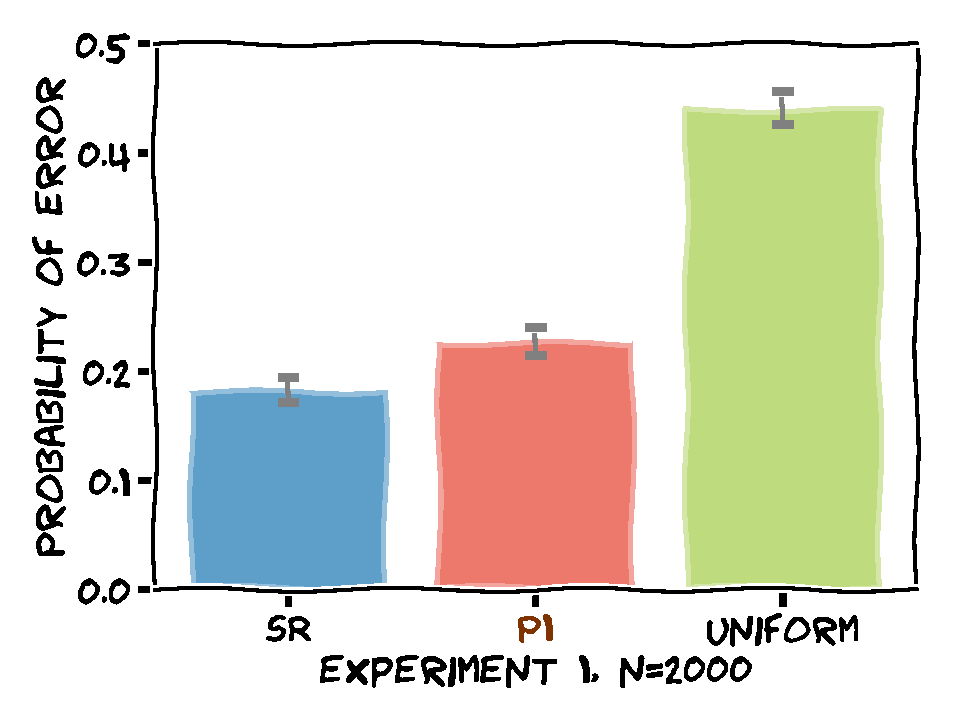
\includegraphics[width =.46\textwidth]{./image/exp1.pdf}$\qquad$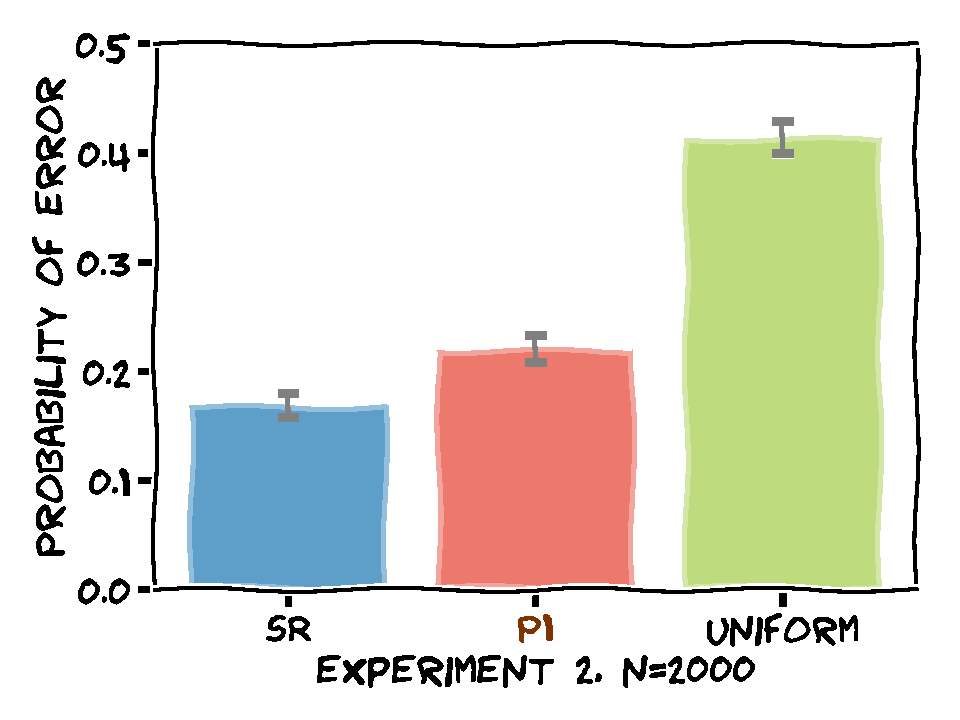
\includegraphics[width =.46\textwidth]{./image/exp2.pdf}
		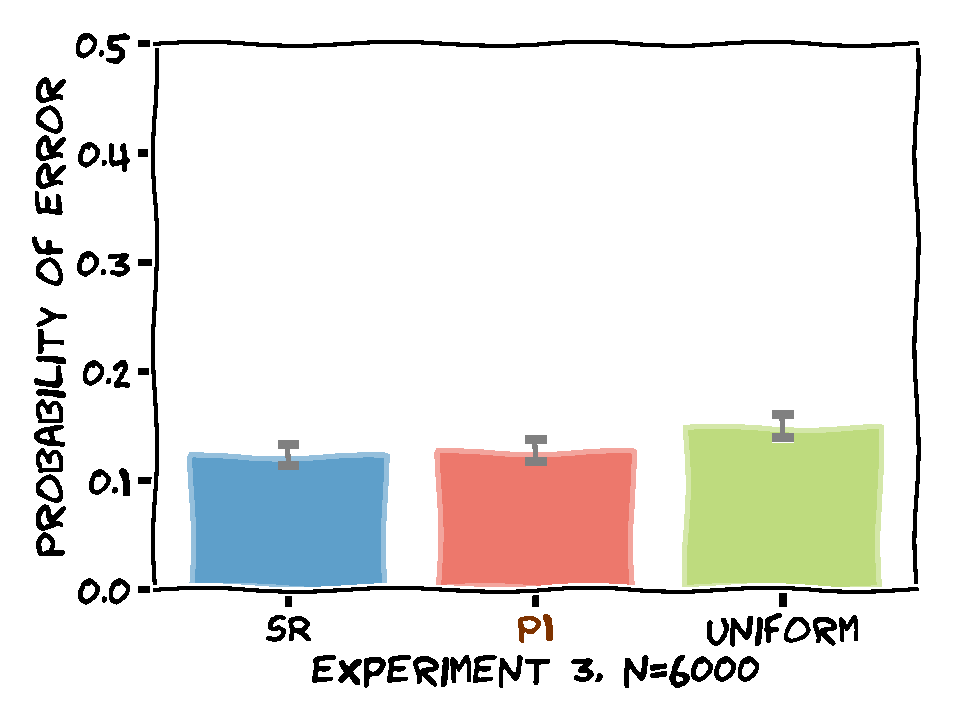
\includegraphics[width =.46\textwidth]{./image/exp3.pdf}$\qquad$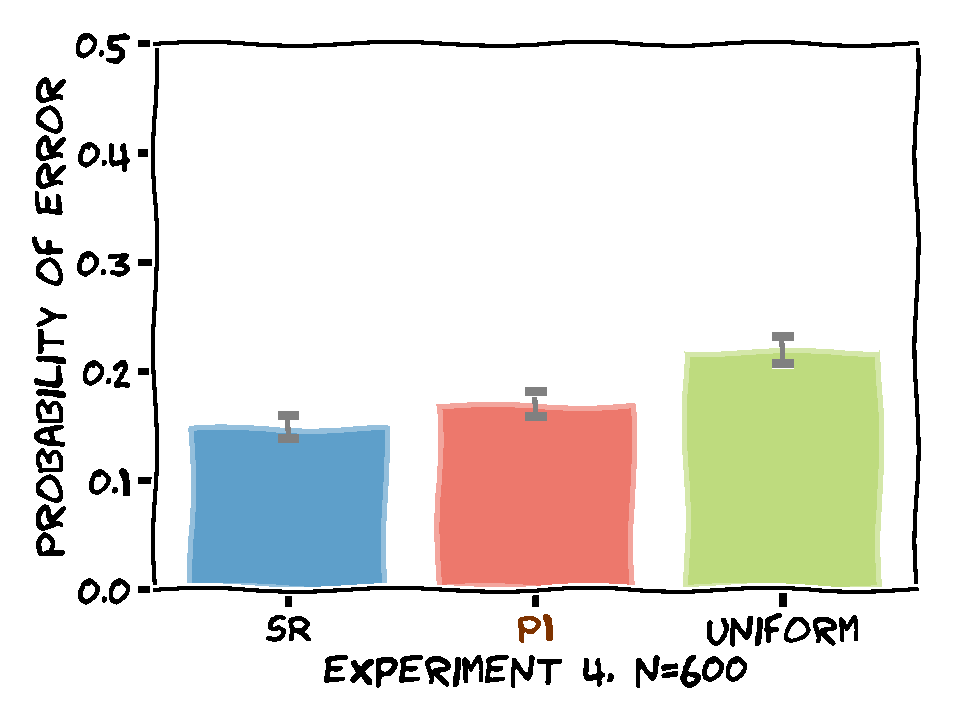
\includegraphics[width =.46\textwidth]{./image/exp4.pdf}
			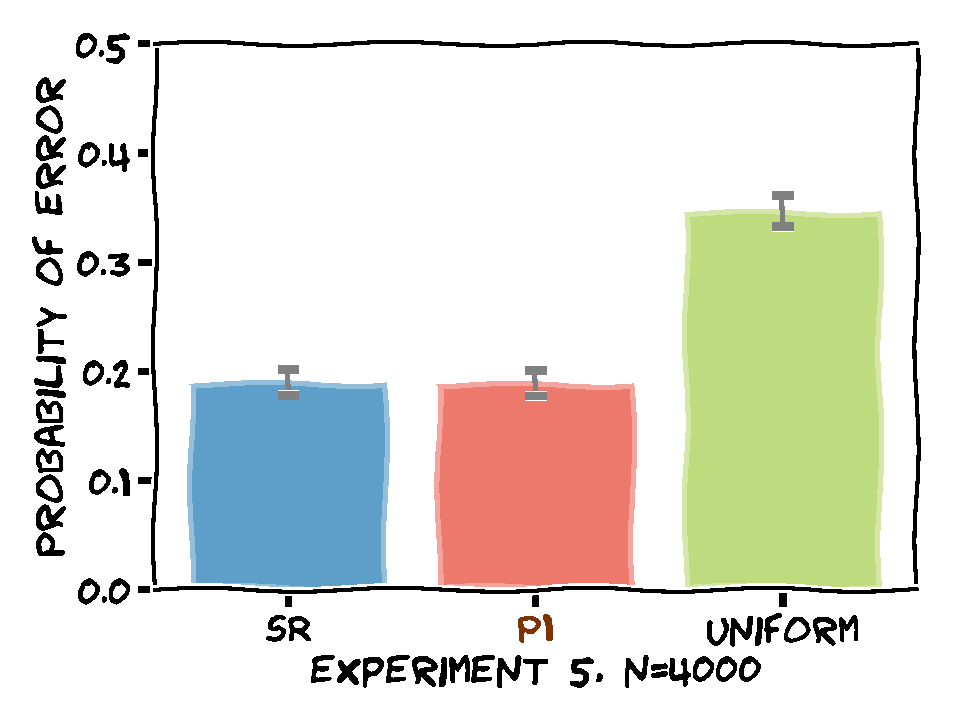
\includegraphics[width =.46\textwidth]{./image/exp5.pdf}$\qquad$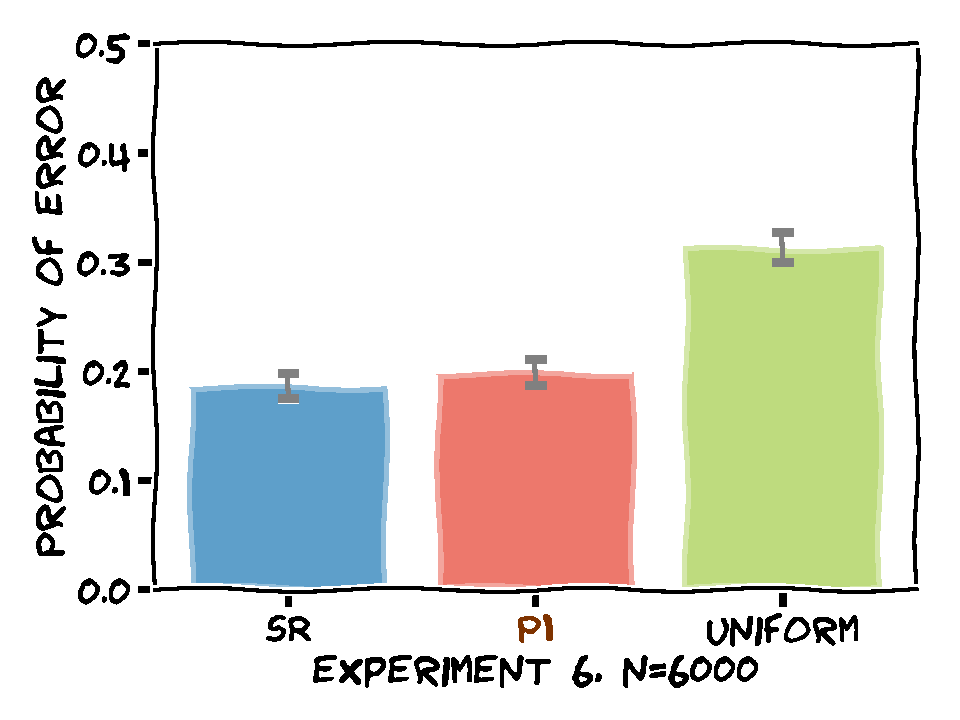
\includegraphics[width =.46\textwidth]{./image/exp6.pdf}
				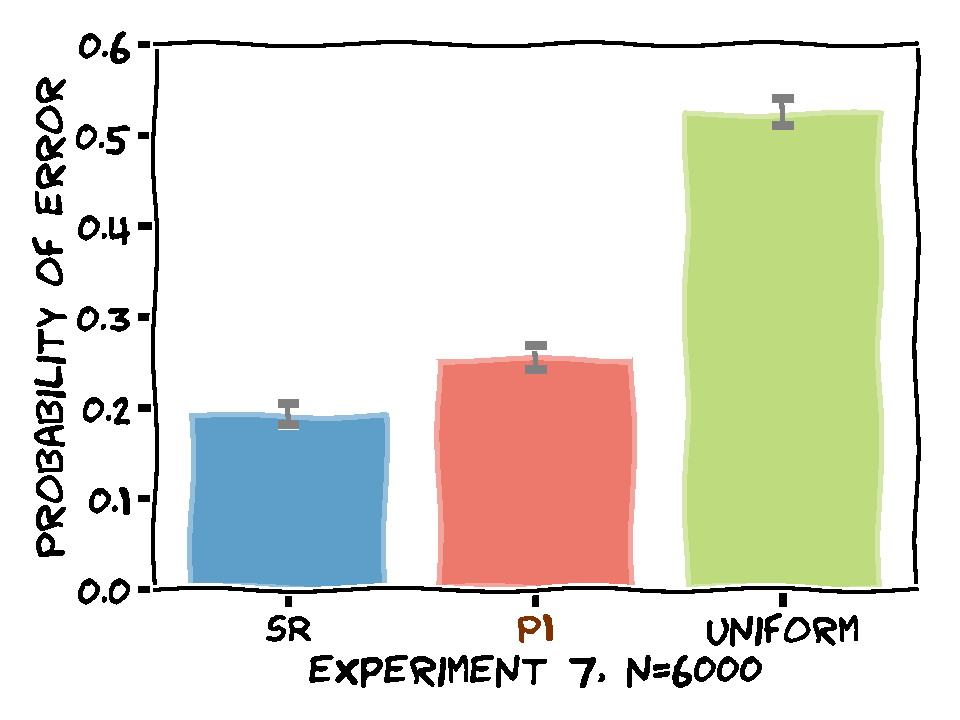
\includegraphics[width =.46\textwidth]{./image/exp7.pdf}$\qquad$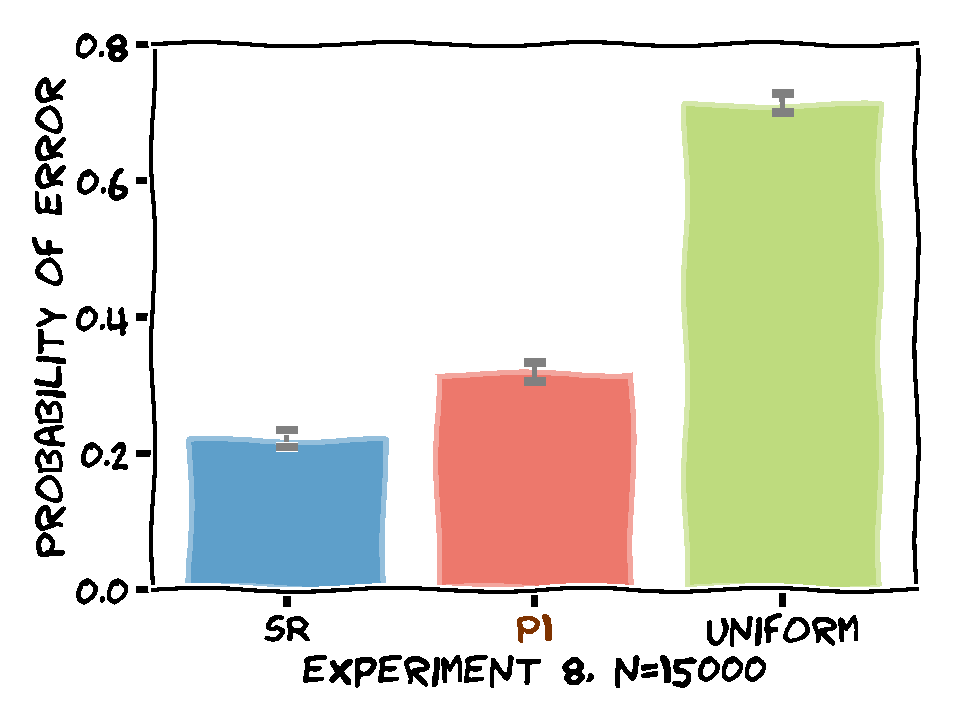
\includegraphics[width =.46\textwidth]{./image/exp8.pdf}
				\caption{Probabilities of error of \SR, \Pone, and the static uniform allocation.}\label{exp}
\end{figure}
